\section{Evaluation}
\label{sec:eval}

{\color{blue} Points to cover:

\begin{itemize}
    \item Local packet detection: Error CDF vs SNR
    \item Diversity gain: Usable spreading factors vs distance/SNR
    \item Impact on client power: Device power trace, Battery life vs distance
    \item Increased capacity due to sensitivity gain (in simulation)
\end{itemize}
}


{\color{blue} }
We implemented our system using 8 LPWAN boards as base stations
distributed across a university campus.  We used a Semtech SX1276 LoRaWAN
transmitter as the client device. We use Charm as the software platform at the
backend to support backhaul. We evaluate our system both through
proof-of-concept experiments and large-scale trace-driven simulations. We
perform our experiments in various environments(both indoors and outdoors) to
ensure the viability of the approach in different situations.

\subsection{Role of Transmission Rates on Battery Life}
\label{sec:energy-savings}

\begin{figure}[!htb]
\centering
\begin{tabular}{@{}c@{}}	
\subfloat[Typical client device current consumption for a complete LoRaWAN transmission. The device is powered at $3V$.]{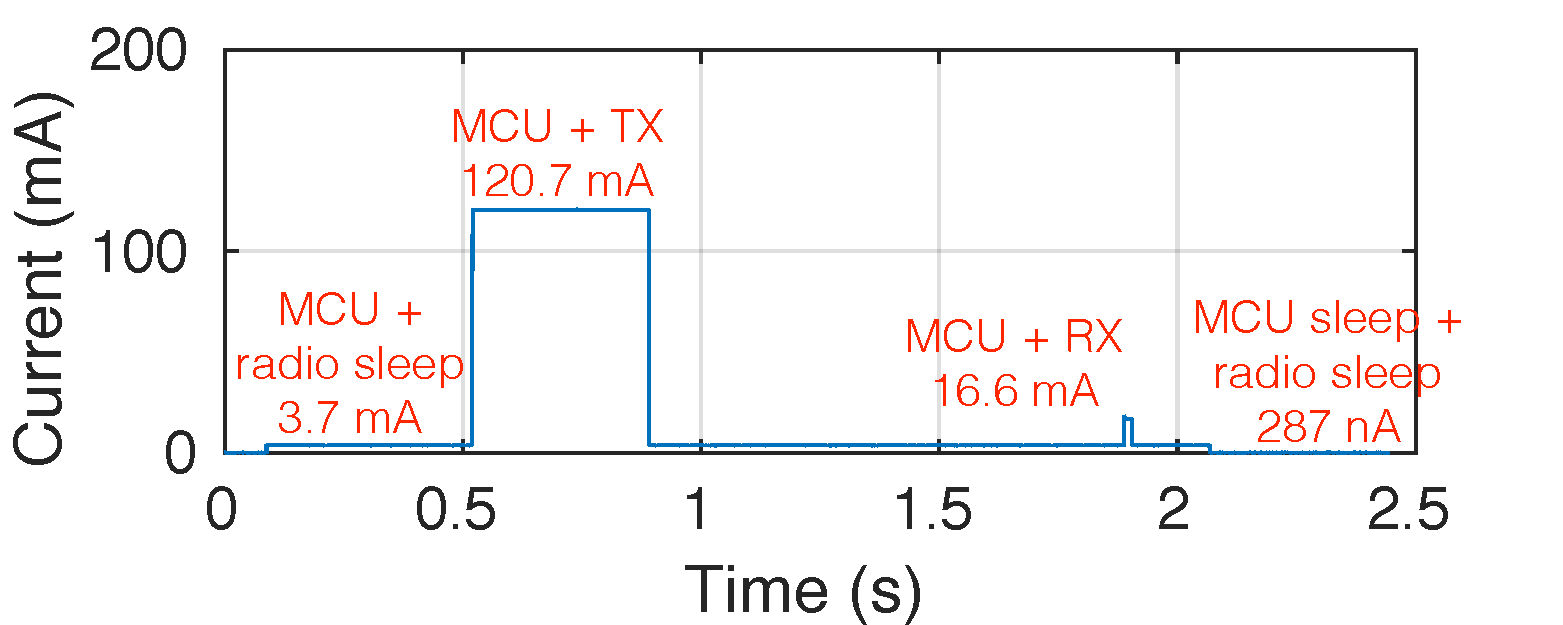
\includegraphics[width=0.4\textwidth]{figures/bug_power_trace_annotated}
\label{fig:power-trace}} \\
\subfloat[Estimated lifetime of a client device powered by two AA batteries sending 36 byte packets at various data rates based on the energy profile.]{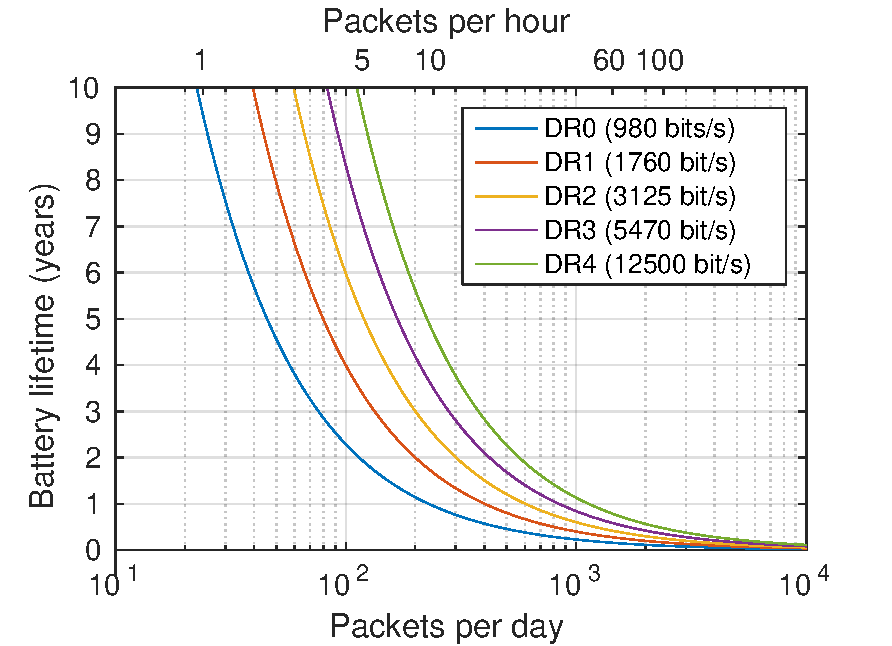
\includegraphics[width=0.4\textwidth]{figures/LoRaBug_AA_lifetime_semilog}
\label{fig:lifetime-estimates}}
\end{tabular}
\caption{}
\end{figure}

Most LP-WAN client devices are expected to be small, low-cost and low-maintenance battery-operated devices performing primarily some sensing functions. As these devices are expected to operate for many years, battery life is a major concern and is very difficult to optimize for. The amount of data to transmit is determined by the device and we do not attempt to alter it in this paper. Similarly, to maintain compatibility, we do not alter the MAC protocols or client device requirements specified in LoRaWAN.

We analyzed the energy profile of a typical client device, shown in \figref{power-trace}. The device performs some local computation, transmits a LoRa message, waits for an acknowledgement from the network and then goes to low-power sleep mode. The radio transmission consumes the highest amount of energy ($= \text{area under the curve} \times \text{voltage}$) by a large margin. Thus, any optimization to battery life must focus on reducing the energy of transmissions.

Two parameters affect the energy consumed by transmissions: (1) transmit power and (2) transmit time. Using the currently available LoRa radio chipsets (Semtech SX1272 and SX1276), we've observed that the transmit power does not significantly change the power drawn from the battery during transmission. Any optimization will thus have to focus on reducing the transmit time. The transmit time is determined by the data rate and the amount of data to send. We do not control the amount of data generated by client devices and thus, improving the data rate would provide the largest improvements.

\figref{lifetime-estimates} shows the estimated battery life of a client device if it were to communicate with different data rates. Wireless systems try to communicate at the highest data rate that does not cause too many errors. In the case of LoRa devices, switching to a slower data rate increases the spreading factor,  which have better sensitivity on the receiver. Thus, LoRa devices communicating at the highest spreading factors (and correspondingly using the lowest data rates) can communicate at much longer range and with higher reliability. The negative effect is a significant increase in their transmission time which severely affects battery life.

Using Charm's joint decoding strategy, we enable devices previously forced to use low data rates due to distance or bad coverage, to communicate at higher data rates and lengthen their battery life. Devices which could previously communicate with at least one base stations using the highest data rate reliably, thus gain no benefit from Charm.

\begin{figure}[!ht]
\centering
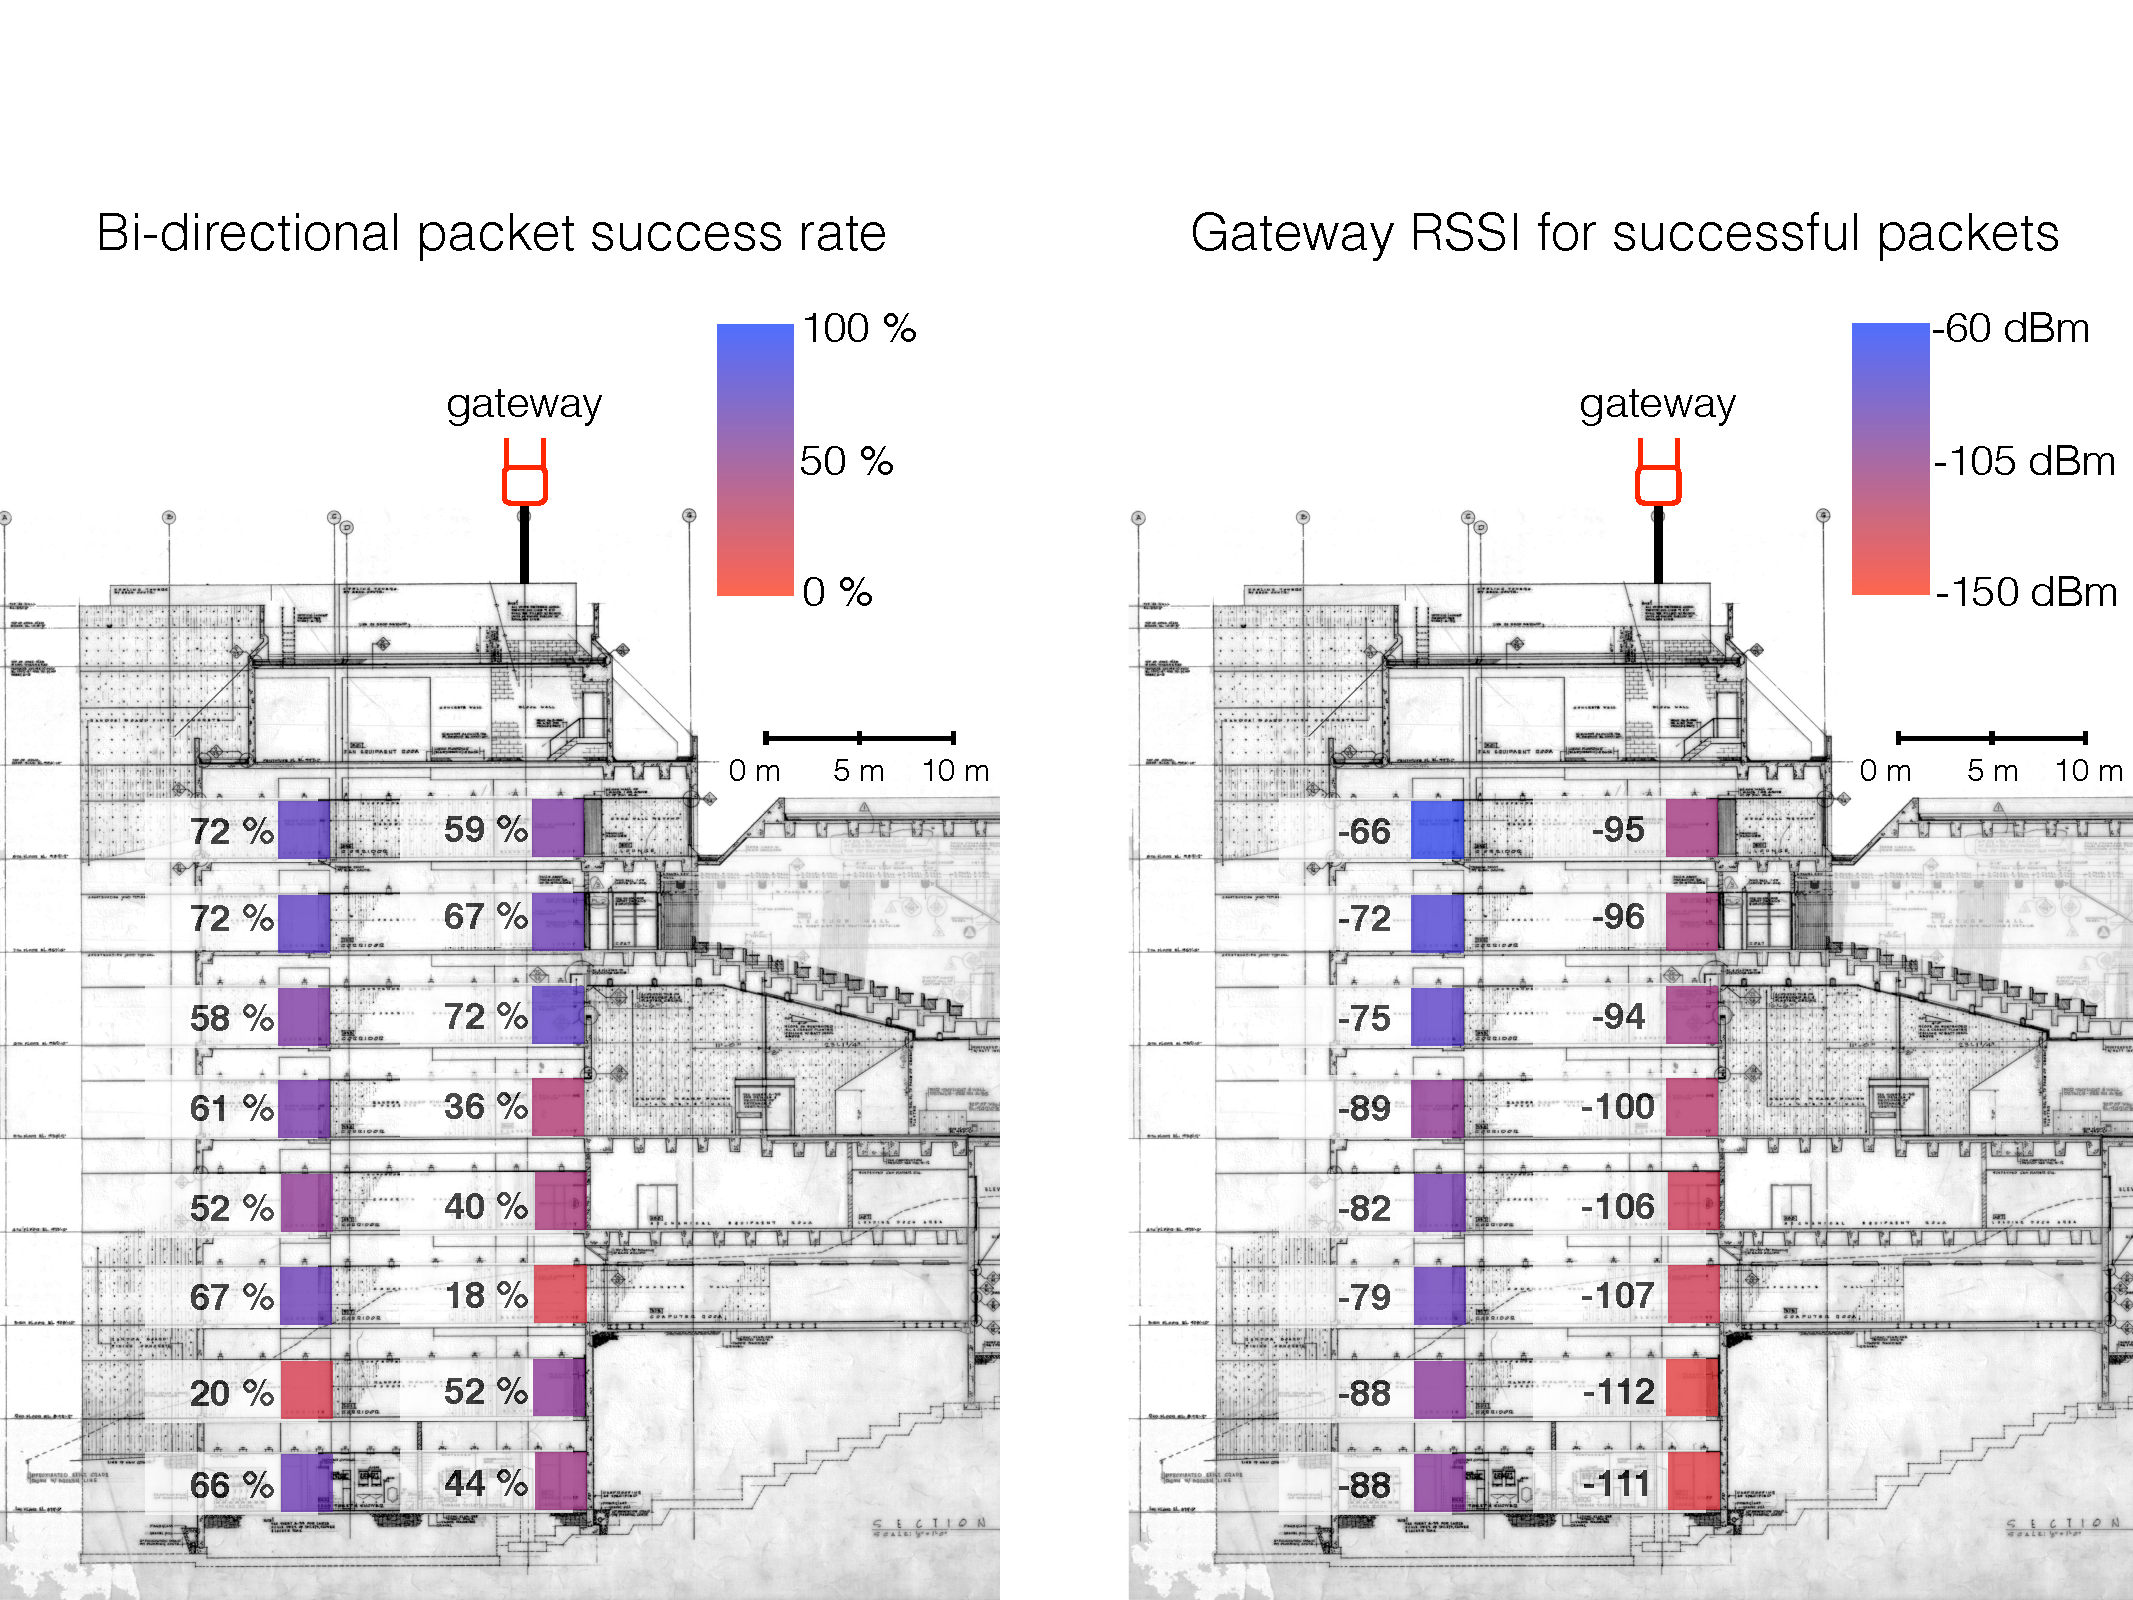
\includegraphics[width=0.45\textwidth]{figures/penetration_test_wean_cropped}
\compactimg
\caption{RF signal penetration experiments performed in a large poured-concrete building. (Left) shows the success rate for bi-directional packet exchange between end-node and gateway and (right) shows the RSSI at the gateway for successful transfers.}
\label{fig:penetration-test}
\end{figure}

This is useful to not only increase coverage but also in urban scenarios with lots of obstructions and devices deep inside buildings. \figref{penetration-test} shows a penetration test experiment inside an on-campus poured-concrete building. Despite a gateway being placed on the roof of the building, we observe the received signal strength to vary as much as 46 dBm at various locations inside the building. A number of client devices, deep inside structure, would have been forced to use the the slowest data rate but can now benefit from Charm.

\subsection{Local detection algorithm}
\label{sec:local-detection-eval}

\begin{figure}[!ht]
\centering
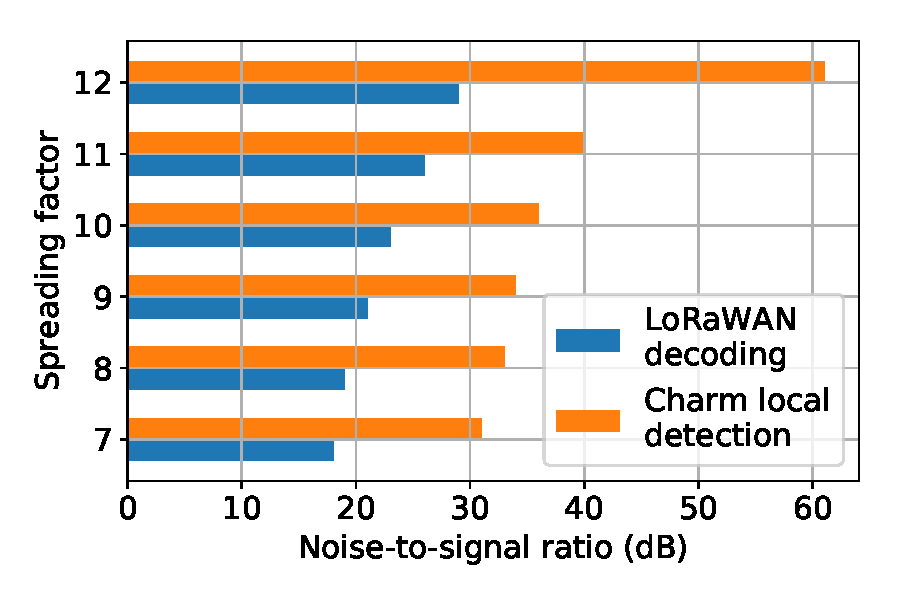
\includegraphics[width=0.45\textwidth]{figures/local_detection_limits}
\caption{{\color{blue} Add caption...}}
\label{fig:local-detection}
\end{figure}

{\color{blue} Akshay, Revathy, Swarun have to describe this

TODO: Add simulation plot.}

Explain why there is a sudden jump from SF11 to SF12 detection?

\subsection{Diversity gain}
\label{sec:diversity-gain-eval}

{\color{blue} Akshay, Revathy, Swarun have to describe this

TODO: add plot of results}

\subsection{Effect on coverage and client data rates}
\label{sec:coverage-data-rate-improvement}

Did some drive tests to calibrate a log distance model

Found our max range is 3.7 km not 10 km in an urban environment

Based on the model, we created a simple simulation to explain 

\begin{figure*}[!htb]
\centering
\subfloat[Dense cells]{
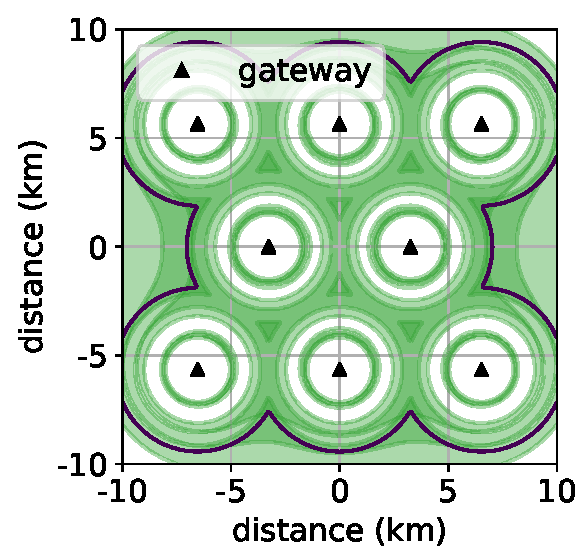
\includegraphics[width=0.3\textwidth]{figures/dense_cells_charm_improvement_cropped}
\label{fig:dense-improvement}
} \hfill
\subfloat[Sparse cells]{
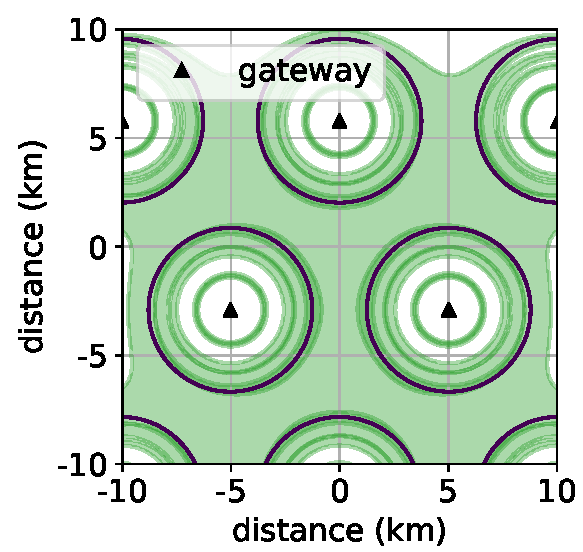
\includegraphics[width=0.3\textwidth]{figures/sparse_cells_charm_improvement_cropped}
\label{fig:sparse-improvement}
} \hfill
\subfloat[Random placement]{
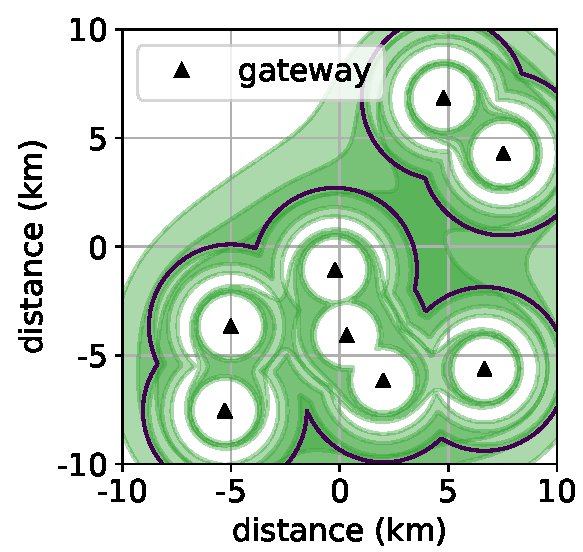
\includegraphics[width=0.3\textwidth]{figures/random_placement_charm_improvement_cropped}
\label{fig:random-improvement}
}
\compactimg
\caption{{\color{blue} (Add caption)}}
\label{fig:charm-improvement}
\compactimg
\end{figure*}